\newcommand{\depiction}[1]{\parbox{0.7cm}{\includegraphics[height=0.7cm]{../assets/depictions/#1.pdf}}}
\newcommand{\depictionSM}[1]{\parbox{0.6cm}{\includegraphics[height=0.6cm]{../assets/depictions/#1.pdf}}}


\section{Experiments and results}

Now that the engine, the tools and the methodology are defined, we can proceed to the experiments. Experiments will be divided in three sections: motivation, experiment and results. The motivation will explain why I think the experiment is relevant and present possible hypothesis. The experiment will describe configurations to train different models, how they will be evaluated and what are my expectations. The results will present the data, explain whether my hypothesis was correct or not and give a brief conclusion. \\

Every model's training configuration is defined by the following variables:

\begin{itemize}
\item \textbf{Feature set}: Determinates the encoding of the position, and thus the number of inputs of the model. It conditions which patterns the network can learn. Experimenting with this is the main focus of this thesis.

\item \textbf{Network architecture}: The size of each layer in the network. The first layer (L1) is the feature transformer and it is efficiently updated. The following layer (L2) should be tiny due the NNUE architecture. The size of the model (its complexity) roughly determinates how many patterns the network can learn.

\item \textbf{Dataset}: The positions to train on. The dataset used is explained in detail in chapter 5. In summary, there are 48.5 billion positions to train on and the dataset remains constant across all runs. About 5 million positions are used for validation.

% no me gusta la palabra computed...
\item \textbf{Training method}: Can choose to use either computed evaluations or PQR triplets. This determinates the format of the samples as well as the loss function. All experiments will train using computed evaluations, unless specified. Explained in detail in chapter 5.

\item \textbf{Training hyperparameters}: The usual machine learning hyperparameters for training, such as batch size, learning rate and scheduler. Recall that each epoch is 100 million positions, and the training will usually last for 1024 epochs.
\end{itemize}

Once training is completed, the models will be evaluated depending on the experiment. To assess the performance a model or to compare a set of models, the following indicators are used:

\begin{itemize}
\item \textbf{Loss}: The training and validation loss are used to detect overfitting and other possible problems. It can't be used to measure the performance of a model. Bigger models must have much better predictions to outweight the cost of having slower inferences and thus lower node visits. It's a tradeoff.

\item \textbf{Puzzle accuracy}: The percentage of moves correctly predicted by the engine in Lichess puzzles. Each puzzle may contain multiple moves, and the engine has 100ms per move.

\item \textbf{Relative ELO rating}: A tournament is played between different models to determine their relative strength. Ordo is used to compute the ELO of each model based on the results of the tournament. This is the most important metric, as it is the most reliable way to measure an engine's strength.

% \item \textbf{Inference performance (infs/s)}:

\item \textbf{Training duration}: The amount of time it takes to train a model. This is a one time operation and it does not affect the performance of a model. However, it does condition which and how many experiments I can run.
\end{itemize}

The experiments are all run in the same hardware: Intel 14900K CPU (24 cores, 32 threads) for dataset generation, batching and evaluation, and a single NVIDIA RTX 4090 24GB GPU for training.

\subsection{Baseline}

\textbf{Motivation.} Experiments that will follow will focus on trying out different feature sets, so it is natural to keep every other variable contant. Since the dataset is fixed and the feature set is the variable, it remains to find acceptable values for the network architecture and the training hyperparameters. 

Due time and resources constraints, I decided to set the training hyperparameters to   (similar) values which give good results in the official Stockfish trainer: \textbf{a batch size of 16384, a learning rate of 0.0005 and a exponential decay factor of 0.99}. This values showed acceptable results during early stages of development and will remain fixed for all runs.

It remains to find a good network architecture. Bigger networks may have lower loss and predict better, but they will also have slower inferences. This is the tradeoff between inference time and node visits (more depth), which are also affected by the quality of the prediction due better prunning. So the model must be so much better to compensate the slowdown in inference. \\

\textbf{Experiment.}  In this first experiment I will try different sizes of L1 and L2,  to find an acceptable tradeoff for future experiments. The feature set used to train will be \featureset{Piece}, the canonical set with 768 features.

I expect that there will be a model that performs best and other models that are smaller (need stronger predictions) and bigger (need speed to visit more nodes) perform worse.

Since I will be running a grid search, I will train the models for 256 epochs (25.6 billion positions) instead of my target of 1024 to make this preliminar process faster. \\

\textbf{Results.} Looking at the result heatmaps in Figure \ref{fig:baseline_heatmaps}, the first thing to notice is that training and validation losses behave as expected. If the model is more complex, meaning the number of parameters (which is dominated by $768*L1+L1*L2$) is higher, the loss is lower and the model predicts better.

When the models are loaded into the engine and evaluated in a tournament, we can see that when L2 drops, the performance drops dramatically. This is due the fact that the inference time is mostly dominated by L2. This result suggests that it may be a good idea explore even lower values of L2, such as 16 or even 8. However, the SIMD implementation requires L2 to be a multiple of 32 so it needs a refactor to keep be fast. So, instead of fiddling with SIMD I decided to \textbf{keep L2 at 32}.

\begin{figure}[h]
\centering
\makebox[\textwidth]{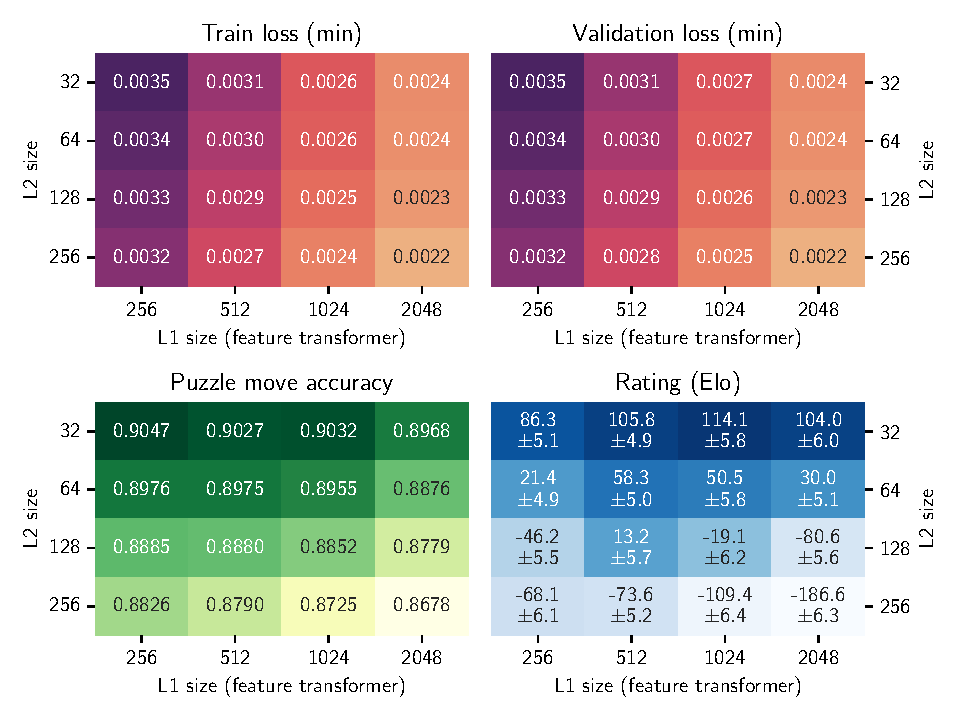
\includegraphics[width=\textwidth]{./dynamic/output/baseline_heatmaps.pdf}}
\captionsetup{justification=centering}
\caption{Network architecture sweep results (L1 $\times$ L2).\\ Ratings computed using $N\approx11000$ games per model. Table in Appendix \ref{appendix:baseline}.}
\label{fig:baseline_heatmaps}
\end{figure}

% L1 e' "gratis", asi que no cambia mucho 

If L2 is kept constant, the best L1 is not the smallest nor biggest.

[escribir elección de L1]

So, further experiments will use a L1=512 and L2=32. The values selected here are specific to the current implementation of the engine, since it may change if more optimizations are made (tradeoff is altered). For reference, Stockfish currently uses L1=2560, and employ more tricks to make it even faster. We can now proceed with more interesting experiments.

\newpage
\subsection{Axis encoding} % relevance
\label{sec:axis_encoding}

\textbf{Motivation.} Looking back at the networks generated by \featureset{Piece} in baseline runs, the learned weigths of most neurons in the feature transformer layer (L1) are related with the movement pattern of the pieces. Let's take the example in Figure \ref{fig:rook_weights}, which depicts the \featureset{Square} part of the features where the role is \symrook\ Rook.

\begin{figure}[h]
\centering
\subfloat[\centering $\white$ White]{{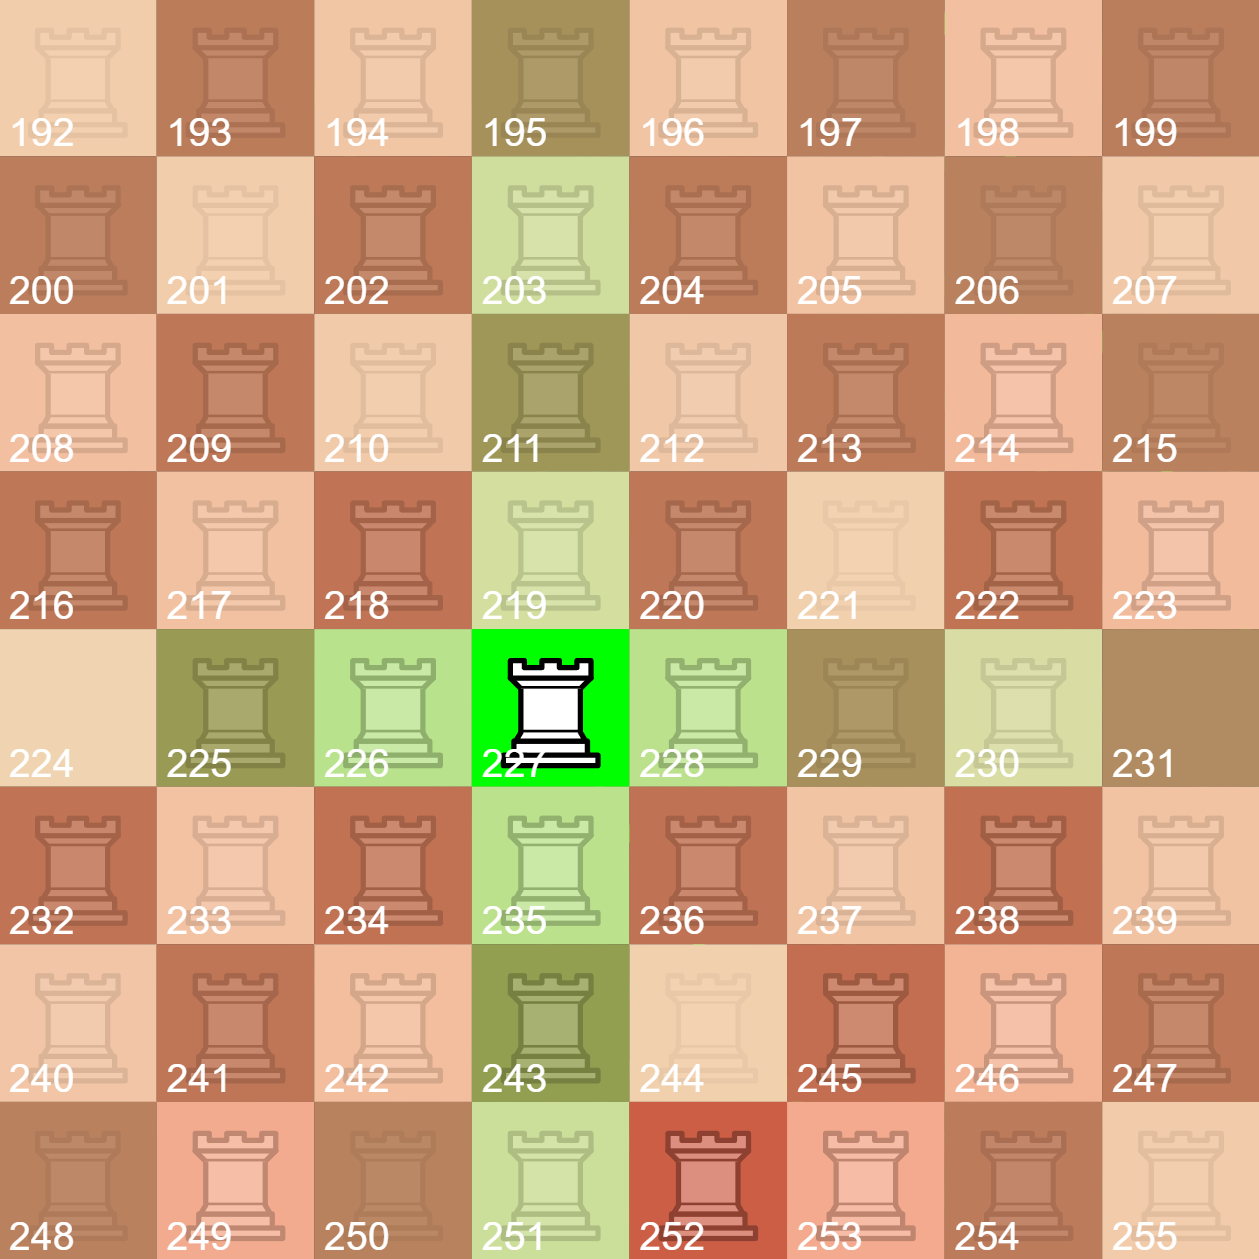
\includegraphics[width=7cm]{../assets/results/piece_weights/white_rook_weights.png} }}%
\qquad
\subfloat[\centering $\black$ Black]{{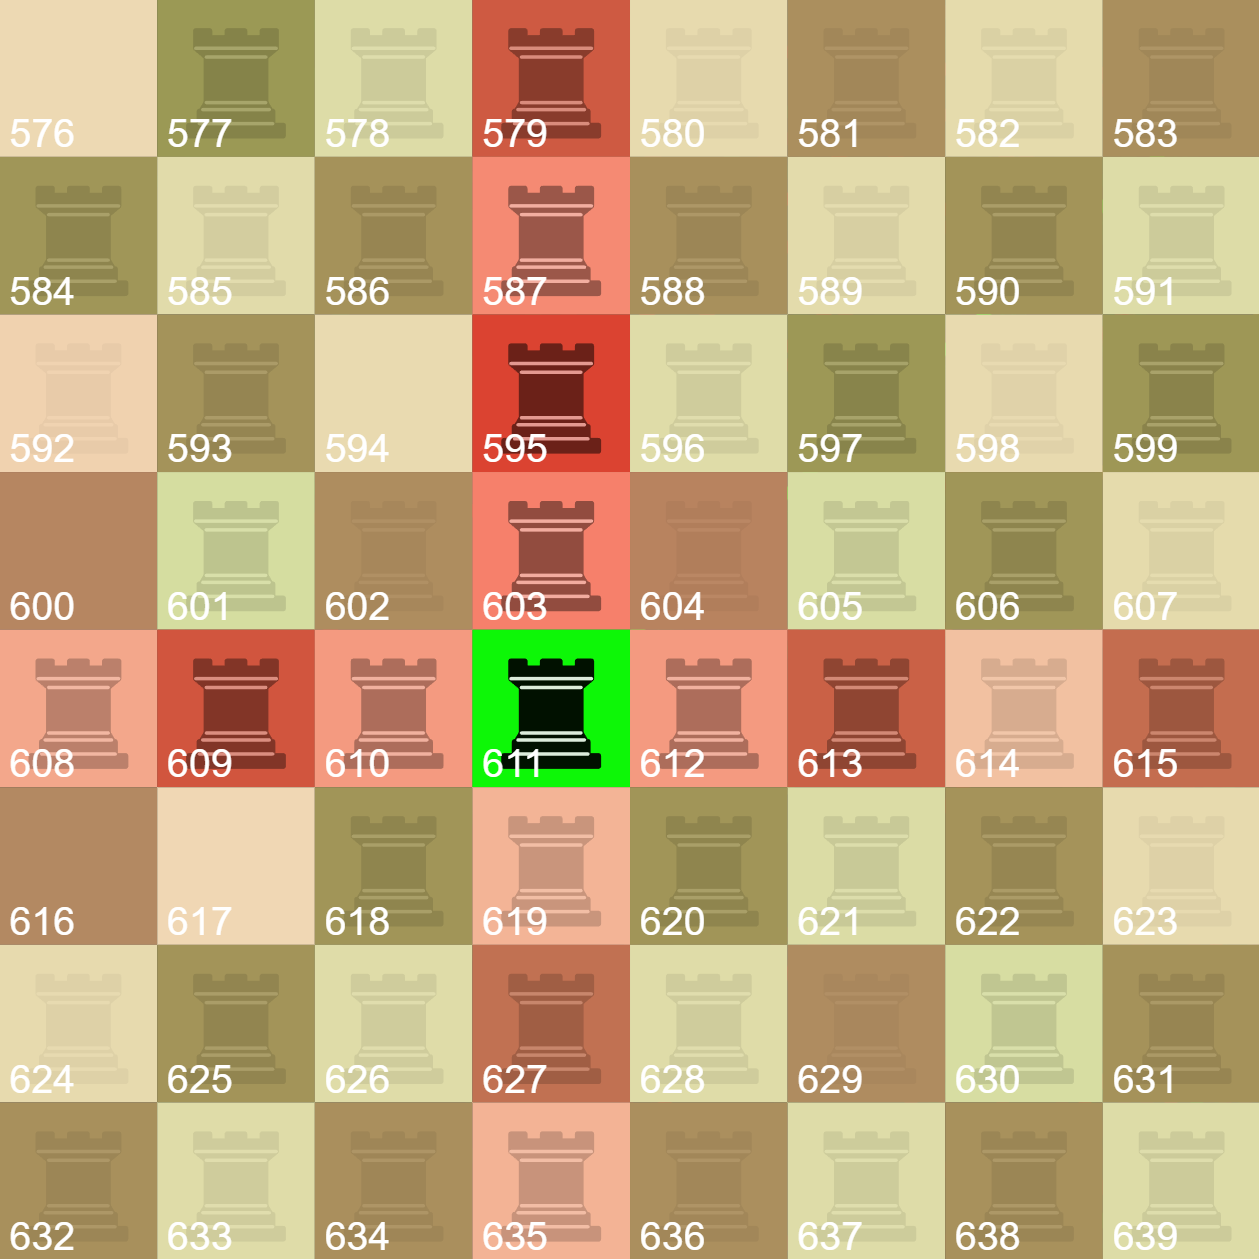
\includegraphics[width=7cm]{../assets/results/piece_weights/black_rook_weights.png} }}%
\caption{Weights of \textbf{a neuron} in the L1 layer, which are connected to features in \featureset{Piece} where the role is $\rook$ Rook. The intensity represents the weight value, and the color represents the sign (although not relevant).}
\label{fig:rook_weights}
\end{figure}

This particular neuron learned to recognize the presence of a rook, affected by the pattern of another potential rook in the same file or rank. Doing so, it had to relate one feature for every potential square where a rook could be for that specific center location, which restrains the network from learning more complex patterns and it is harder to train, because you need more samples to account for all possible combinations.

What if we add a feature which describes \enquote{\textit{there is a $\white$ White $\rook$ Rook in the 4th rank}}? Certainly, this would make the network's job easier, as it would only need to learn the presence of rooks in the corresponding file or rank, instead of every square. This idea can be extrapolated to diagonals, to ease patterns with $\bishop$ Bishops and the $\queen$ Queen.

More examples of this behaviour can be found in Appendix \ref{appendix:axis_samples}, showcasing diagonal patterns and the $\knight$ Knight movements, although they do not move straight through axes. \\

\textbf{Experiment.} I will explore combinations of positional encodings for the pieces on the board, using the available axes. The canonical \featureset{Piece} feature set encodes each piece's position using the square it is located. Note that this is the same thing as encoding the position for a piece $P$ as $\featureset{File}_{P} \times \featureset{Rank}_{P}$. So the position of each piece is determined using the vertical (across ranks) and horizonal (across files) axes.

I will use the natural axes of a chess board:

\begin{table}[H]
\centering
\begin{tabular}{cccc}
\depiction{H} & \depiction{V} & \depiction{D1} & \depiction{D2} \\
Horizontal & Vertical & Diagonal 1 & Diagonal 2 \\
(across files) & (across ranks) &  & 
\end{tabular}
\end{table}

These axes coincide with the movement pattern of the pieces, which make them good candidates to encode the features I proposed. In table \ref{tab:axis_encoding} I present the feature sets that I decided to try. The feature sets are named according to the axes they combine.

\begin{table}[H]
\caption{Axis encoding feature sets\protect\footnotemark}
\label{tab:axis_encoding}
\centering

\newcommand{\rolecolor}{$\times$ $\featureset{R}_{P} \times \featureset{C}_{P}$}

\begin{tabular}{cccccc}
\toprule
\bf Depiction & \bf Feature set & \multicolumn{2}{c}{\makecell{\bf Definition\\for every piece $P$ in the board}} & \bf \makecell{\# of\\features} \\
\toprule
\depiction{H} $\oplus$ \depiction{V} & $\featureset{H} \oplus \featureset{V}$ & $(\featureset{File}_{P} \oplus \featureset{Rank}_{P})$ & \rolecolor & 192 \\
\midrule
\depiction{D1} $\oplus$ \depiction{D2} & $\featureset{D1} \oplus \featureset{D2}$ & $(\featureset{Diag1}_{P} \oplus \featureset{Diag2}_{P})$ & \rolecolor & 360 \\
\midrule
\makecell{\depiction{H} $\oplus$ \depiction{V} $\oplus$ \\ \depiction{D1} $\oplus$ \depiction{D2}} & \makecell{$\featureset{H} \oplus \featureset{V}$ $\oplus$ \\ $\featureset{D1} \oplus \featureset{D2}$} & \makecell{$(\featureset{File}_{P} \oplus \featureset{Rank}_{P}$ $\oplus$ \\ $\featureset{Diag1}_{P} \oplus \featureset{Diag2}_{P})$} & \rolecolor & 552 \\
\midrule
% ------------------------------------
\midrule
\depiction{HV} & \featureset{HV (Piece)} & $\featureset{File}_{P} \times \featureset{Rank}_{P}$ & \rolecolor & 768 \\
\midrule
\depiction{HV} $\oplus$ \depiction{H} $\oplus$ \depiction{V} & $\featureset{HV} \oplus \featureset{H} \oplus \featureset{V}$ & \makecell{$(\featureset{File}_{P} \times \featureset{Rank}_{P}$ $\oplus$ \\ $\featureset{File}_{P} \oplus \featureset{Rank}_{P})$} & \rolecolor & 960 \\
\midrule
\depiction{HV} $\oplus$ \depiction{D1} $\oplus$ \depiction{D2} & $\featureset{HV} \oplus \featureset{D1} \oplus \featureset{D2}$ & \makecell{$(\featureset{File}_{P} \times \featureset{Rank}_{P}$ $\oplus$ \\ $\featureset{Diag1}_{P} \oplus \featureset{Diag2}_{P})$} & \rolecolor & 1128 \\
\midrule
\makecell{\depiction{HV} $\oplus$ \depiction{H} $\oplus$ \depiction{V} \\ \hspace{0.7cm} $\oplus$ \depiction{D1} $\oplus$ \depiction{D2}} & \makecell{\featureset{HV} $\oplus$ \featureset{H} $\oplus$ \featureset{V} \\ $\oplus$ \featureset{D1} $\oplus$ \featureset{D2}} & \makecell{$(\featureset{File}_{P} \times \featureset{Rank}_{P} \oplus$ \\ $\featureset{File}_{P} \oplus \featureset{Rank}_{P}$ $\oplus$ \\ $\featureset{Diag1}_{P} \oplus \featureset{Diag2}_{P})$} & \rolecolor & 1320 \\
\bottomrule

\multicolumn{5}{c}{\footnotesize \textbf{Note:} $\featureset{R}_{P} \times \featureset{C}_{P}$ expands to $\featureset{Role}_{P} \times \featureset{Color}_{P}$}

\end{tabular}

\end{table}

\footnotetext{Note that one could build \depictionSM{D1D2}, \depictionSM{HD1}, \depictionSM{HD2}, \depictionSM{VD1} and \depictionSM{VD2} but they are equivalent to \depictionSM{HV}.}


I expect that the feature sets that are sums of single axes ($\depictionSM{H} \oplus \depictionSM{V}, \depictionSM{D1} \oplus \depictionSM{D2}$ and $\depictionSM{H} \oplus \depictionSM{V} \oplus \depictionSM{D1} \oplus \depictionSM{D2}$) will perform worse overall, since to capture the exact position of pieces in the board, the network will have to learn to relate at least two features for every location. This information is already available when there is a product of two axes (\depictionSM{HV}).

The feature sets that in addition to \depictionSM{HV} include lone axes (\depictionSM{H}, \depictionSM{V}, \depictionSM{D1} and \depictionSM{D2}) should perform better than without, providing that the idea explained in the motivation holds.
Note that even having twice the features, the penalty on inference performance should be minor due L1 being updated efficiently. [saco esto? ya se sabe...]

For each of the proposed feature sets, I will train a network and evaluate its performance relative to each other using a tournament. I expect to see them ranked in the reverse order as presented in the table (more extra axes better). \\

\textbf{Results.} Aca poner los resultados

so........

The next experiment will focus on adding more specific features, instead of more broad ones.


% TODO: change "Piece" to "All" feature set
\featureset{All}

\subsection{Pairwise axes}

Pepito \depiction{PH} asdo \depiction{PV} asd\depiction{PD1} asd\depiction{PD2} asd

3 runs
HV + PH
HV + PV
HV + PH + PV

el cosito de los pares

\subsection{Mobility}

as bitset
as counts

\subsection{Attacks}

as bitsets per piece type
number of attacks

\subsection{Symmetry / Relativity}

\textbf{Motivation.}

BUCKETING

Medir el impacto de agregar simetría al fs. Red mas chica, inf mas rapida, mejor perf?

probar simetria, eventualmente probar con el mejor feature set de arriba, a ver si mejora poniendo a cada bloque individual simetria

\featureset{Half-Relative(H|V|HV)King-Piece}?

inspired by KP, build features relative to the position of the $\king$ King

\subsection{Piece movement}

Intentar capturar los patrones que se ven en P, asi se pueden reconocer patrones mas complejos.
una alternativa es ... la idea de los pares

\featureset{Piece-Move}

Bad perf.

\subsection{Statistical features}

Define \featureset{k-Piece-Piece}

\featureset{King-Piece} is a subset of \featureset{Piece-Piece}.

Top P

Hacer un subset de \featureset{PP} (589824).

\begin{itemize}
\item Destilar?
\item Probar si es lo mismo quedarse con el TOP K de las mas comunes o con las que dice el performance.
\item Catboost? PCA?
\end{itemize}

\subsection{Human behavior}

PQR human behaviour. Medir estilo Maia. comparar? no va a ser tan bueno.




% -----------------
hablar del tradeoff de los feature sets, la primera capa, y demás

vertical and horizontal data, probar dataset sin info vertical u horizonal / ambos y ver que pasa
ver si agregar capas posteriores ayuda o no "layer layers small increase in perf"

measure updates per move average and refreshes average per FS



\subsection{Active neurons}

medir si hay feature sets que no usen neuronas, que esto disparo el uso de HalfTopK

average number of features enabled by feature set (cantidad y porcentaje)



